%%=============================================================================
%% PROOF-OF-CONCEPT
%%=============================================================================

\chapter{\IfLanguageName{dutch}{Werking huidig systeem}{Operation of the current system}}%
\label{ch:current system)}

\section{Inleiding}
\label{sec:inleiding_currsys}
Dit hoofdstuk zal de werking van het huidige systeem om coolgen applicaties te ontwikkelen van ArcelorMittal Gent toelichten en visualiseren. De stappen die in het huidige systeem aanwezig zijn zullen ook terug te vinden zijn in het nieuwe systeem met behulp van een pipeline en IBM DBB. Het is uiterst noodzakelijk om kennis te hebben van het huidige systeem alvorens een nieuw systeem kan gemaakt/geïmplementeerd worden. Dit komt doordat het systeem dat momenteel gebruikt uitermate veel is gepersonaliseerd door ArcelorMittal Gent om aan hun eisen en gebruiken te voldoen. 

\section{Compileren}
\label{sec:compileren}
De huidige geïnstalleerde versie van de Cobol compiler binnen ArcelorMittal Gent is versie 6.20, deze versie van Cobol is geïntroduceerd in 2017 op 8 september en heeft geen support meer vanaf 30 september 2024.
\\ \\
De JCL die uitgevoerd wordt wanneer men een compilatie van een programma wil uitvoeren wordt opgeroepen via een product van Rocket software namelijk MSP (Manager Products). Dit product zorgt ervoor dat een ontwikkelaar kan meegeven welk programma hij/zij wil compileren en in welke omgeving die dat wil doen, dit kan bijvoorbeeld productie of ontwikkeling zijn. Dat product zorgt er dan voor dat de JCL voor de compile uit te voeren wordt gestart met de juiste parameters en de juiste libraries die moeten meegegeven worden tijdens de compilatie zoals de SYSLIB en SYSIN DD's.
\\ \\
Heel belangrijk binnen het huidig systeem is het gebruik van meta-data, hierdoor weet in dit geval MSP welke parameters die moet aanvoeren aan de compiler, welke libraries die moet alloceren en of er extra zaken moeten gestart worden zoals een Db2 package bind of Db2 plan bind. Deze meta-data is dan ook een van de eerste zaken dat gecontroleerd wordt als men een compilatie wil starten. Indien er geen meta-data te vinden is dan zal de compile geannuleerd worden. 
\\ \\
Deze meta-data bevat onder andere informatie over de afdeling waar het gemaakt is, de programmeur van de applicatie, wat voor soort applicatie het is. Zo heb je 3 verschillende soorten programma's binnen ArcelorMittal Gent, je hebt de main programma's, die kunnen ofwel volledig onafhankelijk draaien of ze roepen sub programma's op. Deze main applicaties kunnen zelf niet opgeroepen worden door andere applicaties. Als laatste zijn er ook nog 2 soorten sub programma's, de fsub en de sub. In theorie is er niet veel verschil buiten de manier waarop ze opgeroepen kunnen worden. Zo wordt een sub statisch gebindt aan een programma dat hem oproept en een fsub wordt dynamisch opgeroepen tijdens de run time. Naast die 3 soorten van applicaties is er ook nog het feit of er gebruik gemaakt wordt van subsystemen zoals IMS, Db2 of MQ. Indien hiervan gebruik gemaakt wordt dan kan de ontwikkelaar ook deze zaken aanduiden binnen het meta-data scherm van zijn/haar applicatie. 
\\ \\
Eenmaal alle meta-data aanwezig is zal MSP met behulp van skeletons de juiste JCL opmaken om die applicatie te compileren met de juiste libraries en parameters. De compile parameters zijn heel gelijkaardig voor alle soorten programma's maar kunnen toch nog ergens licht afwijken. Zoals wanneer er gebruik gemaakt wordt van een subsysteem zoals IMS of Db2.
\\ \\

\section{Bind}
\label{sec:bind}
Er wordt gebruik gemaakt van de IEWL Binder voor z/OS 2.5 om de applicaties van ArcelorMittal te binden. Het belangrijkste verschil tussen een programma dat gebind is met IEWL en een dat gelinkedit is, is het feit dat bij de linkedit een groot uitvoerbaar bestand gemaakt wordt van de verschillende objectbestanden van het hoofdprogramma, de subprogramma's en de subroutines die opgeroepen worden. Hierdoor is het programma dat gelinkedit wordt statisch aangemaakt, dit wil zeggen dat indien er een sub programma verandert er dus een nieuwe linkedit moet gebeuren van alle progamma's die dat sub programma gebruiken. Met een binder kan je dynamisch een programma aan een ander programma koppelen/binden, op die manier is het zo dat een sub programma opgeroepen wordt op run time en niet tijdens de compile. Hierdoor hoeft er geen herlink meer te gebeuren van de applicaties die dat programma gebruiken. 
\\ \\
Er zijn net zoals bij de compilatie ook parameters die meegegeven worden aan de binder om op de juiste manier de programma's te kunnen binden. In tegenstelling als bij de compilatie moet er niet voor elk soort programma (main, Db2, IMS, sub, ...) een aparte parameter lijst gemaakt worden. De parameters zijn hetzelfde voor main- en fsub programma's aangezien die worden opgeslagen als DLL, voor de sub programma's is er een andere parameter lijst die ervoor zorgt dat de sub geen DLL wordt maar statisch blijft. Hierdoor zullen main- en fsub programma's wel dynamisch opgeroepen kunnen worden tijdens run time en zal er voor sub programma's opnieuw met herlink en hercompile moeten gewerkt worden. 
\\ \\ 
De binder wordt net zoals de compiler opgeroepen door het product MSP, het gaat op dezelfde manier te werk als bij de compile en maakt gebruik van een applicatie zijn meta-data om zo de juiste libraries en parameters mee te geven.

\chapter{Proof Of Concept}
\label{ch:poc}

\section{Inleiding}
\label{sec:inleiding_poc}
Het hoofdstuk van de Proof Of Concept zal gaan over welke stappen en producten er allemaal nodig waren om de proefopstelling succesvol te laten werken. Deze stappen zullen overeenkomen met die van het huidige systeem besproken in het vorige hoofdstuk.
\\ \\

\section{Installatie \& configuratie IBM DBB}
\label{sec:installdbb}
De eerste stap in het opzetten van de proefopstelling is om de IBM DBB installatie af te ronden en de configuratie te starten. De installatie op de mainframe van ArcelorMittal werd gedaan door een bedrijf genaamd NRB, zij zijn verantwoordelijk voor installatie van software op de mainframe van ArcelorMittal Gent. 
\\ \\
Aangezien IBM DBB al geïnstalleerd is voor deze Proof Of Concept kan er direct begonnen worden aan de configuratie van de bestanden die gebruikt worden door het product DBB. Deze bestanden zijn onder andere properties bestanden die ervoor zorgen dat bepaalde zaken zoals de binder en compiler worden gedeclareerd. Deze zijn niet standaard meegeleverd en moeten afgehaald worden vanaf een git repository namelijk de dbb-zappbuild git repository van IBM. 
\\ \\
\subsection{Installatie dbb-zappbuild}
Die repository kan rechtstreeks gecloned worden of via file transfer kunnen die ook op de juiste plaats in de USS belanden. De aanbevolen plaats om die repository te stockeren is in de hoofdfolder van DBB, dat ziet eruit zoals /dbb/dbb-zappbuild.
\\ \\
\subsection{Configuratie dbb-zappbuild}
Nu dat de dbb-zappbuild repository aanwezig is op de USS kan er begonnen worden aan de configuratie van DBB. Deze configuratie op de USS bestaat hoofdzakelijk uit properties en .groovy bestanden. De properties bestanden zijn te vinden in de folder build-conf en zijn ook de eerste die moeten veranderd of ingevuld worden. Verder zijn er de .groovy bestanden die voor de verwerking van die properties zorgen, dit is in een hoofdprogramma (build.groovy), language specifieke programma's zoals Cobol.groovy en utility programma's zoals BuildUtilities.groovy.
\\ \\
Deze bestanden hebben elk hun eigen taken en nut in de werking van het systeem, zo zijn de properties bestanden noodzakelijk om datasets en PDS'en mee te geven om zo de juiste binder, compiler, load libraries en dergelijke te hebben. De taak van een language specifiek groovy programma zoals Cobol.groovy is om de compilatie en bind van een programma dat in die taal geschreven is uit te voeren. Dit kan heel erg verschillen tussen talen door, zo is de compilatie van een PL/I programma een stuk anders dan de compilatie van een Cobol programma. De zaken die nodig zijn om die compilatie en bind goed uit te voeren kunnen gevonden worden in zo'n language specifiek groovy programma. Deze language specifieke programma's gebruiken heel vaak utility programma's om zaken die hetzelfde zijn in elke taal te bundelen zo is er een BindUtilities.groovy dat een DB2 package bind en/of plan bind kan doen. Dit is onafhankelijk van welke taal je gebruikt en kan dus in zo'n utility programma. Als laatste om de cyclus te vervolledigen is er de build.groovy, dit is het hoofdprogramma dat alle andere programma's op de juiste moment oproept.
\\ \\
\begin{figure}[h]
\begin{tabularx}{1\textwidth} { 
        | >{\centering\arraybackslash}X 
        | >{\centering\arraybackslash}X 
        | >{\centering\arraybackslash}X 
        | >{\centering\arraybackslash}X  | }
    \hline
    Properties bestanden & 
    Language groovy bestanden & 
    Utility groovy bestanden & 
    build.groovy \\
    \hline
    Dataset en PDS declaratie & 
    Oproepen van utilities en language specifieke werking bepalen & 
    Werking van language onafhankelijke procedures bepalen & 
    Oproepen van de juiste groovy sub programma's \\ 
    \hline
\end{tabularx}
\caption{Soorten bestanden en hun taak}
\label{tab:soorten bestanden}
\end{figure}

\subsubsection{Properties bestanden}
Er zijn in totaal 16 properties bestanden waarin aanpassingen moeten aangebracht worden deze zijn onderverdeeld in de verschillende talen en gebruiken. Zo zijn er properties bestanden voor Cobol, PL/I, PSB, ACB en nog een aantal anderen. Er is ook een datasets.properties bestand waarin veel algemene PDS'en en datasets worden gedeclareerd. Zo kan je bijvoorbeeld de z/OS macro library, Cobol compiler, PL/I compiler en DB2 load library vinden en declareren in de datasets.properties. 
\\ \\
In de build.properties zit er vooral algemene instellingen en dus geen datasets, zo kan je aanduiden welke properties bestanden ingeladen kunnen worden als het systeem geactiveerd word. Deze zit net zoals de datasets.properties en de overige taal- en gebruiksspecifieke properties bestanden in de build-conf folder die te vinden is binnen de dbb-zappbuild map. 
\\ \\
De taal specifieke properties worden aangepast in onder andere Cobol.properties en de PLI.properties bestanden. Hierin worden onder andere instellingen zoals load libraries, vereiste properties en compiler opties meegegeven die algemeen gelden voor alle programma's van die taal. De volledige properties bestanden zijn te vinden in appendix \ref{ch:appropsbuild}.
\\ \\
\subsubsection{Language groovy bestanden}
De language groovy bestanden zorgen ervoor dat de programma's van die taal succesvol gecompileerd en gebind kunnen worden. Naast de compile en bind wordt er ook gezorgd dat de load module van de applicatie op de juiste plaats beland, dat er een DB2 package bind en/of plan bind uitgevoerd wordt indien nodig. Zo wordt ervoor gezorgd dat het programma niet alleen goed wordt gecompileerd en gebind maar ook uitvoerbaar is op het mainframe van ArcelorMittal Gent. Binnen dit onderzoek is het enigste language groovy programma de Cobol.groovy, het volledige aangepaste script is te vinden in appendix \ref{ch:aplangroovy}.
\\ \\
\subsubsection{Utility groovy bestanden}
De utility groovy programma's worden door zowel de language groovy bestanden als de build.groovy opgeroepen om language onafhankelijke procedures op te roepen. Zo is er een groovy utility programma dat ervoor zorgt dat onder andere de build lijst wordt aangemaakt, meta data wordt ingevuld, logicalfiles worden aangemaakt en ervoor zorgt dat datasets kunnen aangemaakt worden. Dit is maar een kleine opsomming van de mogelijkheden van de BuildUtility.groovy, hiernaast zijn er nog 7 andere groovy utility programma's. De enigste programma's die aangepast zijn in het kader van het onderzoek zijn BuildUtilities.groovy en BindUtilities.groovy, deze zijn te vinden in appendix \ref{ch:aputilgroovy}. 
\\ \\
\subsubsection{build.groovy}
Dit groovy programma roept andere programma's op zoals de utility programma's en de language specifieke programma's. Er wordt een build lijst gemaakt op basis van de rangschikking die meegegeven wordt binnen de properties van de build. Er worden dus groovy bestanden aangeroepen en de properties worden ingeladen zodat die gebruikt kunnen worden door de build.groovy en de andere groovy programma's. 
\\ \\
Hieronder een opsomming van alle bestanden en programma's die ervoor zorgen dat DBB de programma's en bestanden kan compileren, binden en opslaan in een z/OS omgeving.
\begin{multicols}{2}
    \begin{itemize}
        \item \textbf{Properties bestanden}
        \begin{itemize}
            \item ACBgen.properties
            \item Assembler.properties
            \item build.properties
            \item Cobol.properties
            \item datasets.properties
            \item DBDgen.properties
            \item defaultzAppBuildConf.properties
            \item dependencyReport.properties
            \item LinkEdit.properties
            \item MFS.properties
            \item PLI.properties
            \item PSBgen.properties
            \item Transfer.properties
            \item ZunitConfig.properties
        \end{itemize}
        
        \item \textbf{Language groovy bestanden}
        \begin{itemize}
            \item Assembler.groovy
            \item Cobol.groovy
            \item DBDgen.groovy
            \item LinkEdit.groovy
            \item MFS.groovy
            \item PLI.groovy
            \item PSBgen.groovy
            \item Transfer.groovy
            \item ZunitConfig.groovy
        \end{itemize}
        
        \item \textbf{Utility groovy bestanden}
        \begin{itemize}
            \item BindUtilities.groovy
            \item BuildUtilities.groovy
            \item BuildReportUtilities.groovy
            \item DependencyScannerUtilities.groovy
            \item FilePropUtilities.groovy
            \item GitUtilities.groovy
            \item ImpactUtilities.groovy
            \item ReportingUtilities.groovy
        \end{itemize}
        
        \item \textbf{build.groovy}
    \end{itemize}
\end{multicols}
\\ \\
\subsection{Configuratie DBB buiten USS}
Naast de configuratie van DBB in de zapp-build op USS is er ook een configuratie die in elke repository meegegeven moet worden bij het starten van DBB. Dat zijn properties bestanden die in de repository meegeleverd moeten worden om de compilatie en bind in goed uit te voeren. Deze properties bestanden hebben altijd een application.properties en een file.properties, hierin wordt er onder meer een build lijst rangschikking meegegeven om te beslissen in welke orde programma's zullen gecompileerd worden. Naast de application- en file.properties moet er ook per taal een properties bestand meegegeven worden met extra instellingen die toegevoegd worden aan de al beschikbare instellingen die in de properties op USS zijn gedeclareerd. Zo moet er bij de verwerking van een Cobol programma de file-, application- en Cobol.properties bestanden aanwezig zijn binnen de repository. 
\\ \\
Er zijn in totaal voor ArcelorMittal 10 properties bestanden die meegegeven kunnen worden binnen een repository. Deze worden hieronder opgesomd.
\begin{multicols}{2}
    \begin{itemize}
        \item application.properties
        \item Assembler.properties
        \item Cobol.properties
        \item file.properties
        \item languageConfigurationMapping
        \item LinkEdit.properties
        \item PLI.properties
        \item reports.properties
        \item Transfer.properties
        \item ZunitConfig.properties
    \end{itemize}
\end{multicols}
\\ \\
Naast de properties bestanden is er nog een .gitattributes bestand dat heel belangrijk is in verband met het omzetten van de encodering van z/OS naar git en omgekeerd. Op de mainframe van ArcelorMittal Gent wordt er gebruik gemaakt van de EBCIDIC IBM 1148 encodering en die is niet standaard ondersteund door git. Daardoor moet er in een .gitattributes bestand aangegeven worden dat de input in die EBCIDIC encodering staat en dus nog moet omgezet worden naar UTF-8. De properties bestanden en .gitattributes die gebruikt worden binnen de repository van dit onderzoek zijn volledig aangepast terug te vinden in appendix \ref{ch:appropappli}. 

\pagebreak

\section{Opzetten pipeline Azure DevOps}
Om de compilatie en bind van programma's te voltooien wordt er gebruik gemaakt van pipelines en pipeline software om dat proces te starten. In dit onderzoek zal er gebruik gemaakt worden van Azure Pipelines, een product uit de Azure DevOps suite. De reden dat er gebruik gemaakt wordt van Azure Pipelines en niet van een andere pipeline software zoals Jenkins is door het feit dat ArcelorMittal Gent al een licentie had voor Azure DevOps. Zo wordt de software stack van ArcelorMittal niet onnodig uitgebreid. 

\subsection{Azure DevOps workflow}
Voordat er gestart kan worden moet er bekeken worden welke workflow er gebruikt zal worden binnen de pipeline en Azure DevOps. De workflow die gebruikt wordt in dit onderzoek is heel standaard en zal gaan van een desktop met IDz of Visual Studio Code naar het eindstation z/OS. Dit gaat als volgt te werk, er wordt begonnen vanaf niks dus er is nog geen enkele repository die op de desktop staat. 
\\ \\
De eerste stap is dus om een repository te clonen naar een lokale map, dit kan rechtstreeks vanuit IDz of Visual Studio Code. Dan wordt die repository lokaal aangepast door bijvoorbeeld een nieuwe branch toe te voegen, nieuwe commits of nieuwe code. Als de repository klaar is om doorgestuurd te worden naar z/OS dan wordt er via een ``git push'' een signaal verstuurd naar de centrale repository en die zal dan op zijn beurt een of meerdere pipeline jobs lanceren die uitgevoerd worden door een agent die ofwel op Linux of Windows draait. Die pipeline job zal de repository gaan clonen op z/OS, daarna wordt die repository met behulp van IBM DBB gebuild en de bekomen load modules en source files worden daarna op z/OS opgeslagen. De visuele weergave van deze workflow is te vinden op figuur \ref{fig:azure devops flow}.
\begin{figure}[h]
    \centering
    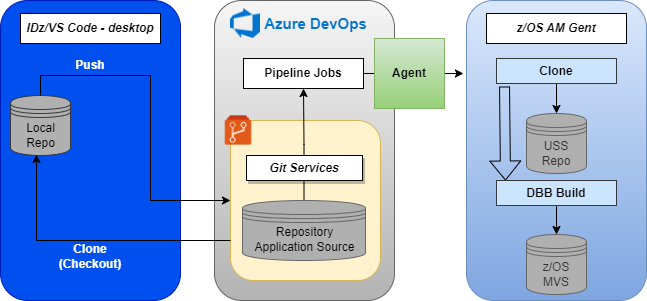
\includegraphics[scale=0.65]{AzureDevOps_Flow}
    \caption{Azure DevOps workflow}
    \label{fig:azure devops flow}
\end{figure}

\subsection{Opzetten van een organisatie in Azure DevOps}








